\chapter{Allgemeines}
%\addcontentsline{toc}{section}{Allgemeines}
%\setcounter{section}{1}
%\setcounter{equation}{0}
\section{Einführung}
Das vorliegende Flughandbuch wurde erstellt, um Piloten und Ausbildern alle notwendigen Informationen für einen sicheren, zweckmäßigen und leistungsoptimierten Betrieb des Motorseglers B13 zu geben.\\
\newline
Das Handbuch enthält zunächst alle Daten die dem Piloten aufgrund der Bauvorschrift JAR-22 zur Verfügung stehen müssen. Es enthält darüber hinaus jedoch eine Reihe weiterer Daten und Betriebshinweise, die aus Herstellersicht für den Piloten von Nutzen sein können.

\section{Zulassungsbasis}
Der Motorsegler B13 wird im Rahmen einer "`Vorläufigen Verkehrszulassung"' betrieben. Die Zulassungsbasis stellt die JAR-22 vom 15. März 1982.\\
\newline
Lufttüchtigkeitsgruppe: Utility
\newpage
\section{Hinweisstellen}
Für die Flugsicherheit oder Handhabung besonders bedeutsame Handbuchaussagen sind durch Voranstellung eines der nachfolgenden Begriffe besonders hervorgehoben:\\
\newline
\newline
\begin{color}{red}
\large{\underline{Warnung}}\\
bedeutet, dass die Nichteinhaltung einer entsprechend gekennzeichneten Verfahrensvorschrift zu einer unmittelbaren oder erheblichen Beeinträchtigung der Flugsicherheit führt.
\end{color}\\
\newline
\begin{color}{forestgreen}
\large{\underline{Wichtiger Hinweis}}\\
bedeutet, dass die Nichteinhaltung einer entsprechend gekennzeichneten Verfahrensvorschrift zu einer geringfügigen oder einer mehr oder weniger langfristig eintretenden Beeinträchtigung der Flugsicherheit führt.
\end{color}\\
\newline
\begin{color}{blue}
\large{\underline{Anmerkung}}\\
soll die Aufmerksamkeit auf Sachverhalte lenken, die nicht unmittelbar mit der Sicherheit zusammenhängen, die aber wichtig oder ungewöhnlich sind.
\end{color}

\section{Beschreibung und technische Daten}
Die B13 ist ein doppelsitziger Motorsegler mit einem gedämpften T-Leitwerk, 4-teiligen Tragflächen, nebeneinander angeordneten Sitzen, Schempp-Hirth Oberseiten-Bremsklappen und einem gefederten Hauptfahrwerk.\\
\newline
Die B13 wurde für wissenschaftliche Zwecke und für den Leistungsflug entworfen.
\newpage
\textbf{Technische Daten}\\

\begin{longtable}{l l l}
Besatzung & & 1+1\\
 & & \\
 Tragflügel & & \\
  & Spannweite & $23,20m$\\
  & Fläche & $18,95m^2$\\
  & Streckung & $28,4$ \\
  & Ersatzflügeltiefe & $873mm$ \\
  & Einstellwinkel & $0^{\circ}$ \\
  & Pfeilung zur $25\%$-Linie & $-0,3^{\circ}$ \\
  & V-Stellung & $1^{\circ}$\\
  & Verwindung & $0^{\circ}$\\
  & Profil & HQ 41/14,35\\
  & Klappentiefe & $17,5\%$ \\
  & & \\
 Rumpf & & \\
 & Länge & $8,55m$\\
 & Breite & $1,28m$\\
 & Höhe & $0,90m$ \\
 & & \\
 Höhenleitwerk & & \\
 & Spannweite & $3,10m$\\
 & Fläche & $1,457m^2$\\
 & Profil & FX 71-L-150/25 \\
 & & \\
 Seitenleitwerk & & \\
 & Höhe & $1,70m$ \\
 & Fläche & $1,71m^2$\\
 & Profil & FX 71-L-150/30\\
 & & \\
 Bremsklappen & & \\
 & Spannweite & $1,50m$\\
 & Höhe & $158mm$ \\
 & Fläche & $0,442m^2$\\
 & & \\
 Fahrwerk & & \\
 & Hauptrad, einziehbar & $380$x$150, 3-3,5Bar$\\
 & Heckrad, fest & $210$x$65, 2,5-2,8Bar$\\
 & Radstand & $5,60m$\\
 & & \\
 Triebwerk & & nicht eingebaut\\
 & & \\
 Massen & & \\
 & Leermasse & s. Wägebericht\\
 & Höchstmasse & $820kg$\\
 & Flächenbelastung min/max & $34,7\frac{kg}{m^2}$/$43,3\frac{kg}{m^2}$\\
 & & \\
 Flugleistungen & bei Flugmasse $765kg$ & \\
 & beste Gleitzahl (WK +1) & $45,4 (95\frac{km}{h})$ \\
 & geringstes Sinken (WK +1) & $0,56\frac{m}{s} (90\frac{km}{h})$

\end{longtable}

\section{Dreiseitenansicht}
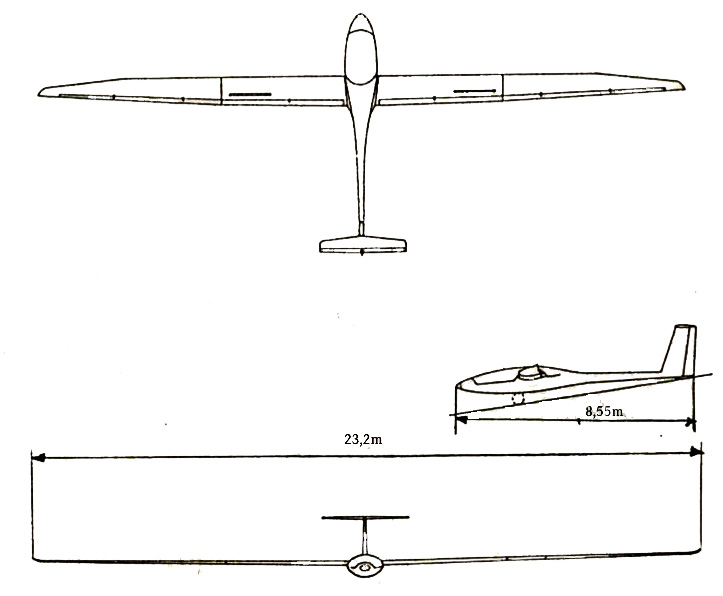
\includegraphics[width=\textwidth]{3seiten.jpg}